\documentclass{standalone}
\usepackage{preset}
\begin{document}
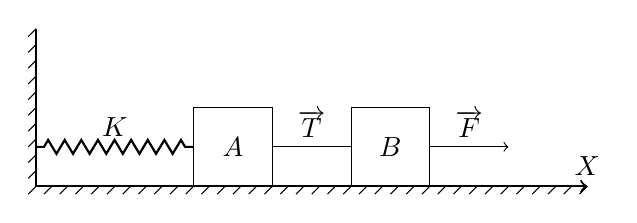
\begin{tikzpicture}[x=10mm,y=10mm]
	\tikzstyle{spring}=[thick,decorate,decoration={zigzag,pre length=0.1cm,post length=0.1cm,segment length=6}]
	\draw[thick](0,0)--(0,2);
	\draw[thick,->](0,0)--(7,0)node[above]{$X$};
	\draw[spring](0,.5)--node[above]{$K$}(2,.5);
	\draw(2,0)rectangle node{$A$}(3,1);
	\draw(3,.5)--node[above]{$\overrightarrow T$}(4,.5);
	\draw(4,0)rectangle node{$B$}(5,1);
	\draw[->](5,.5)--node[above]{$\overrightarrow F$}(6,.5);
	\foreach \x in {.2,.4,...,7}{
		\draw(\x,0)--+(-.1,-.1);
	}
	\foreach \y in {0,.2,...,2}{
		\draw(0,\y)--+(-.1,-.1);
	}
\end{tikzpicture}
\end{document}
